\documentclass[UTF8, a4paper]{ctexart}
\usepackage{fix-cm}
\usepackage{titlesec}
\usepackage{graphicx}
\usepackage{amsmath}
\usepackage{mathtools}
\usepackage{tabularx}
\usepackage{tikz}
\usepackage{listings}
\usepackage{xcolor}
\usetikzlibrary{shapes.geometric, arrows.meta, positioning}
\usepackage[top=2cm, bottom=2cm, left=2cm, right=2cm]{geometry}
% 设置节标题左对齐
\titleformat{\section}[block]{\normalfont\Large\bfseries}{\thesection}{1em}{}

\title{光子探测效率及能谱测量}
\author{夏泽宇}

\begin{document}
\maketitle
\section{计算模型介绍}
\begin{figure}[h]
    \centering
    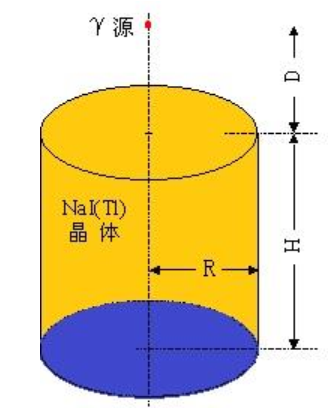
\includegraphics[width=0.2\textwidth]{../fig/model.png}
    \caption{模型图}
    \label{fig:model}
\end{figure}
\begin{itemize}
    \item 闪烁体尺寸$\Phi4\times4 cm$,即半径$R=2cm$、高$H=4cm$
    \item $\prescript{137}{}{Cs}$点源在闪烁体中轴线上,与闪烁体顶面距离$D=20cm$,粒子垂直向下入射进入晶体
\end{itemize}

光子由$\gamma$源射出,进入闪烁体后通过模拟随机过程,最终或者射出闪烁体,
或者因为能量耗尽(发生光电效应或康普顿散射)而被闪烁体吸收。通过统计闪烁体吸收的能量,
并模拟加上正态分布的噪声,得到能谱与其他统计量。

\section{模拟过程}
\begin{tikzpicture}[node distance=2.5cm and 2cm, auto]

    % Define style for different elements
    \tikzstyle{startstop} = [rectangle, rounded corners, minimum width=3cm, minimum height=1cm, text centered, draw=black, fill=red!30]
    \tikzstyle{process} = [rectangle, minimum width=3cm, minimum height=1cm, text centered, draw=black, fill=orange!30]
    \tikzstyle{decision} = [diamond, aspect=2, minimum width=3cm, minimum height=1cm, text centered, draw=black, fill=green!30]
    \tikzstyle{arrow} = [thick,->,>=stealth]

    % Place nodes
    \node (step1) [decision] {光子在闪烁体内部且能量>0?};
    \node (step2) [process, below of=step1, yshift=-1cm] {模拟一次输运过程};
    \node (step3) [decision, below of=step2, yshift=-2cm] {随机取输运距离,更新位置。在闪烁体内部?};
    \node (step4) [decision, below of=step3, yshift=-2cm] {发生光电效应?};
    \node (step5) [process, left=of step4, xshift=-1cm] {能量置为0};
    \node (step6) [process, right=of step4, xshift=1cm] {康普顿散射,更新能量};
    \node (step7) [process, above of=step6] {更新运动方向};
    \node (return) [startstop, left of=step1, xshift=-4cm] {返回能量损失};

    % Draw arrows
    \draw [arrow] (step1) -- node[anchor=east] {是} (step2);
    \draw [arrow] (step1) -- node[anchor=south] {否} (return);
    \draw [arrow] (step2) -- (step3);
    \draw [arrow] (step3) -| node[anchor=east] {否} (return);
    \draw [arrow] (step3) -- node[anchor=east] {是} (step4);
    \draw [arrow] (step4) -- node[anchor=south] {是} (step5);
    \draw [arrow] (step4) -- node[anchor=south] {否} (step6);
    \draw [arrow] (step5) -- (step1);
    \draw [arrow] (step6) -- (step7);
    \draw [arrow] (step7) |- (step1);

\end{tikzpicture}

以上程序模拟了一次输运过程,即光子从入射到出射/吸收的过程。
每次输运过程结束后,统计光子的能量损失,并附加上由于探测器造成的正态分布的噪声,得到最终的能谱与统计量。


代码示例:
% 设置代码样式
\definecolor{deepgreen}{rgb}{0.0, 0.4, 0.0}
\lstset{
    language=Python,                  % 设置语言
    basicstyle=\ttfamily\normalsize, % 设置字体样式
    keywordstyle=\color{blue},         % 关键字颜色
    stringstyle=\color{orange},           % 字符串颜色
    % commentstyle=\color{deepgreen},        % 注释颜色
    morecomment=[l][\color{magenta}]{\#}
}
% 展示代码
\begin{lstlisting}
    # 模拟一次输运过程
    photon = Photon(np.array([0, 0, H]), E0, np.array([0, 0, -1]), H=H, R=2)
    E_D = photon.simulate()
    # 仅统计探测器可识别的光子
    if E_D > 0:
        # 探测器识别数量+1 
        Nm += 1
        E_Ds.append(E_D)
        # 加入探测器的噪声
        F = 0.01 + 0.05 * np.sqrt(E_D + 0.4 * E_D ** 2)
        sigma = 0.4247 * F
        x = np.random.randn()
        E_Detects.append(E_D + sigma * x)   
        
\end{lstlisting}

\section{模拟结果}

\subsection{探测效率、峰总比和相对误差}
探测效率:$N_m/N=61.486\%$

峰总比:$N_p/N=21.119\%$

误差估计:
\[
    \varepsilon=\left|\hat{\eta}_N-\eta\right|<\frac{\chi_\alpha \sigma_\eta}{\sqrt{N}} \approx \frac{2 \sigma_\eta}{\sqrt{N}}
\]

其中:
\[
    \sigma_\eta^2=\eta(1-\eta)=\hat{\eta}_N\left(1-\hat{\eta}_N\right)
\]

代入值$N=10^5$, $\hat{\eta}_N=0.61486$,得到$\varepsilon=3.078\times10^{-3}$,相对误差为$\frac{\varepsilon}{N_m/N}=5.005\times10^{-3}$。

\subsection{能谱图}
\begin{figure}[h]
    \centering
    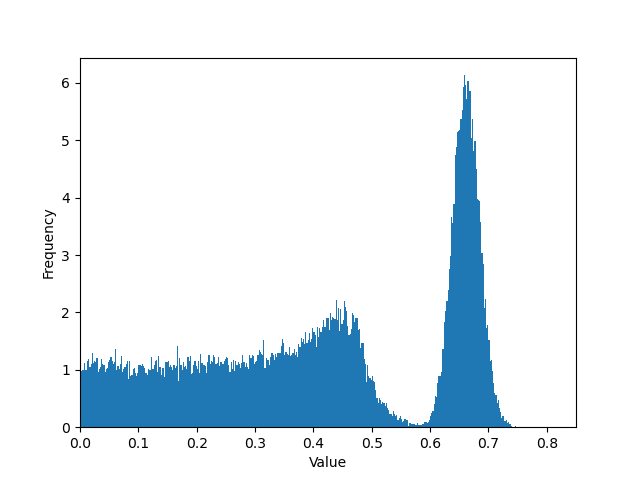
\includegraphics[width=1\textwidth]{../fig/E_D_distribution.png}
    \caption{能谱图}
    \label{fig:energy_distribution}
\end{figure}
\clearpage

\subsection{系统在0.662MeV处的能量分辨率}
考察$\gamma$能谱图的半高宽,即能量分辨率:
\begin{figure}[h]
    \centering
    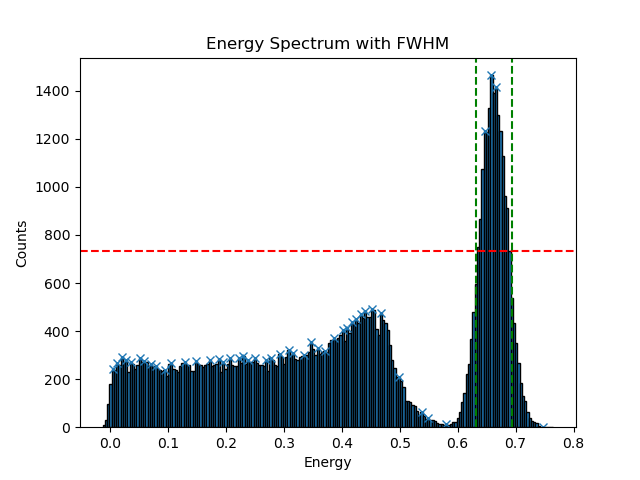
\includegraphics[width=1\textwidth]{../fig/E_D_spectrum_with_FWHM.png}
    \caption{能谱图的半高宽}
    \label{fig:energy_fhwm}
\end{figure}

通过对数据的计算得到,半高宽对应的区间为$[0.6311, 0.6934]$,因此能量分辨率为:
\[
    \frac{0.6934-0.6311}{0.662}=9.4\%
\]

可以看出该光子探测器的能量分辨率较低,主要原因在于测量系统引入了过多误差。

\section{总结}
通过对光子探测系统的模拟,可以得到探测效率、峰总比和能量分辨率等信息。
就模拟得到的数据,该系统的探测效率、峰总比、能量分辨率均不太高。
可以通过增大设备尺寸,选用更好的探测材料以提高探测效率和峰总比。
能量分辨率的提高则需要提升测量系统的精度。
\end{document}

